\documentclass[a4paper, 12pt, titlepage]{article}
\usepackage[utf8]{inputenc}
\usepackage{geometry}
\usepackage{polski}
\usepackage{graphicx}
\usepackage{float}
\usepackage{etoolbox,refcount}
\usepackage{multicol}
\usepackage{fancyhdr}
\pagestyle{fancy}
\title{Prototypowanie serwomechanizmu dla zespołu napędowego.}
\author{Adrian Jałoszewski, Tomasz Kotowski}
\date{}
\newgeometry{left=2.5cm, right=2.5cm, bottom=2.5cm, top=2.5cm}

\begin{document}
	\maketitle
	\section{Cel ćwiczenia}
		Celem ćwiczenie było stworzenie regulatora trójpołożeniowego oraz PID przy pomocy Simulinka oraz panelu operatorskiego w oprogramowaniu dSPACE do obsługi serwomechanizmu.
	\section{Wykonanie regulatorów w Simulinku}
		Pierwszy regulator stworzony przez nas miał postać jak na poniższym schemacie. Jest to jednak bardzo niepraktyczny model, gdyż oprogramowanie dSPACE nie pozwala na proste wykonywanie operacji arytmetycznych na poszczegoonych wartościach.
		\begin{figure}[H]
			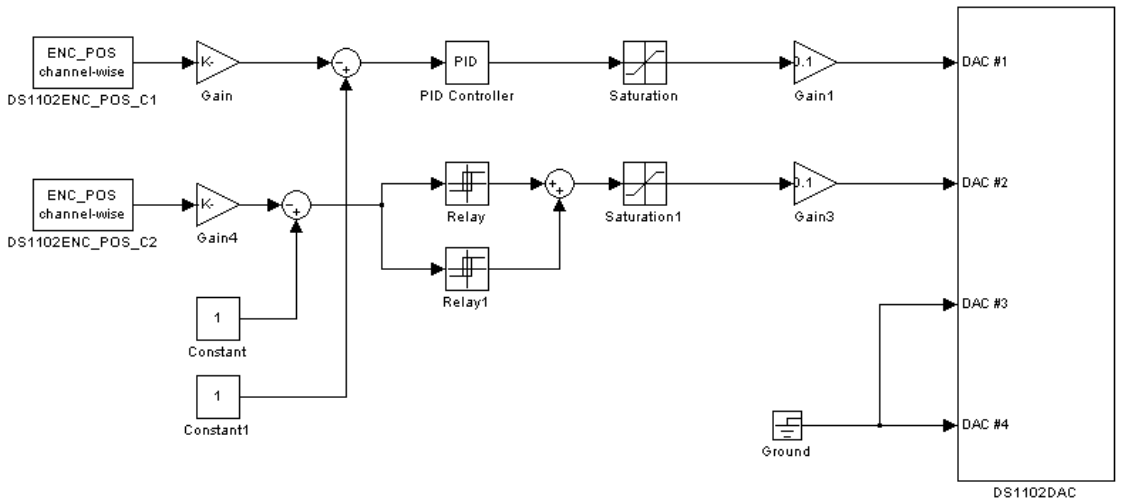
\includegraphics[width=\textwidth]{img/original_system.png}
			\caption{Oryginalny model}
		\end{figure} \noindent
		Zmodyfikowaliśmy więc drugi z bloczków Relay tak aby miał odwrotne miał odwróconą dziedzinę i przeciwdziedzinę -- użyliśmy do tego dwa bloczki odwracające sygnał.
		\begin{figure}[H]
			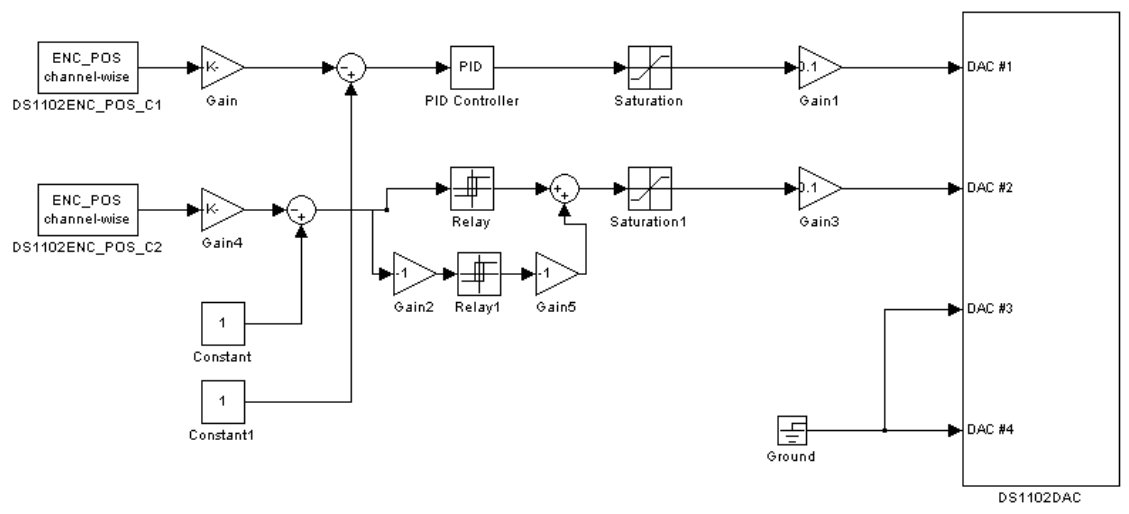
\includegraphics[width=\textwidth]{img/our_improved_system.png}
			\caption{Model z naszymi ulepszeniami}
		\end{figure} \noindent
		Wyjściem bloczków relay jest maksymalny dostępny sygnał jakim jest $+5$. Wartości na wyjściu i na wejściu regulatora są przeskalowane tak aby były dopasowane do rzeczywistego układu.
	\section{Wykonanie panelu operatorskiego}
		Obydwa sygnały wejściowe podpięliśmy do jednego suwaka tak aby można było wprowadzać te same zmiany dla obydwu układów regulacji. Panel ten pozwala na regulację parametrów regulatora PID oraz wartości dla jakiej włącza i wyłącza się regulator trójpołożeniowy.
		\begin{figure}[H]
			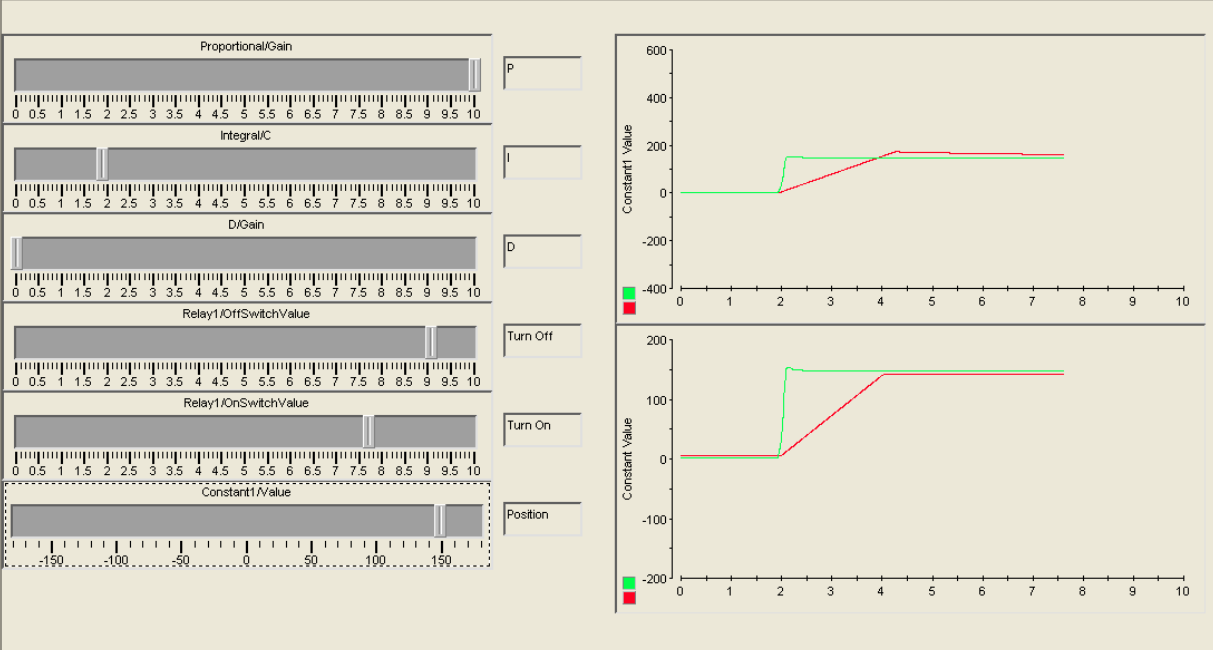
\includegraphics[width=\textwidth]{img/operational_panel.png}
			\caption{Panel operatorski}
		\end{figure}\noindent
		Górny wykres przedstawia odpowiedź na zmianę zadanego położenia dla regulatora PID, dolny pokazuje to samo, tyle, że dla regulatora trójpołożeniowego.
	\section{Wnioski i podsumowanie}
		Laboratorium te przybliżyło nam realizację sterowania obiektem rzeczywistym przy pomocy regulatora stworzonego używając oprogramowania Simulink. Sposób realizacji ćwiczenia natomiast pozwolił nam na równoczesne obserwowanie reakcji obydwu regulatorów na dane wymuszenie. Przez dobieranie przez nas odpowiednich nastaw byliśmy w stanie zaobserwować jak reaguje układ oscylujący oraz układ niestabilny.
\end{document}